\chapter{Example System 2: Thermal Energy Storage}\label{example-system-2-thermal-energy-storage}

This system will detail the process required to model a Plant Loop coupled with Thermal Energy Storage (TES) in EnergyPlus. The input file for this example can be found under the name: PlantApplicationsGuide\_Example2.idf.

The TES tank will be charged by using a chiller loop, which will in turn be cooled by a condenser loop. The schedules for this system are setup such that the TES tank will be charged by the chiller during the night and then the stored chilled water is used to satisfy the building cooling load during the day. The TES tank used in this system is a stratified tank. This system also includes one heating loop which satisfies the heating load. The cooling and heating system operate in conjunction with an air loop that is spread across a total of five zones. The air loop modeling will not be discussed in this guide. This system consists of a total of three separate plant loops, the cooling side is comprised of two loops and the heating side contains one loop. A simple line diagram for the cooling system is provided in Figure~\ref{fig:simple-line-diagram-for-cooling-system}. The EnergyPlus line diagram for the cooling loop is provided in Figure~\ref{fig:energyplus-line-diagram-for-cooling-system}. A simple line diagram for the heating loop is provided in Figure~\ref{fig:simple-line-diagram-for-heating-loop}, whereas its EnergyPlus line diagram is provided in Figure~\ref{fig:energyplus-line-diagram-for-heating-loop}.

\begin{figure}[htbp] % fig 41
\centering
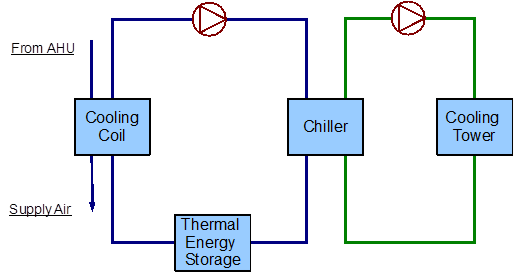
\includegraphics{media/image041.png}
\caption{Simple line diagram for cooling system \protect \label{fig:simple-line-diagram-for-cooling-system}}
\end{figure}

\begin{figure}[htbp] % fig 42
\centering
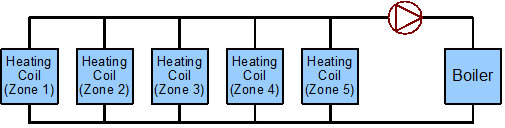
\includegraphics{media/image042.png}
\caption{Simple line diagram for heating loop \protect \label{fig:simple-line-diagram-for-heating-loop}}
\end{figure}

\begin{figure}[hbtp] % fig 43
\centering

\includegraphics[width=0.9\textwidth, height=0.9\textheight, keepaspectratio=true]{media/image043.png}
\caption{EnergyPlus line diagram for cooling system \protect \label{fig:energyplus-line-diagram-for-cooling-system}}
\end{figure}

\begin{figure}[hbtp] % fig 44
\centering
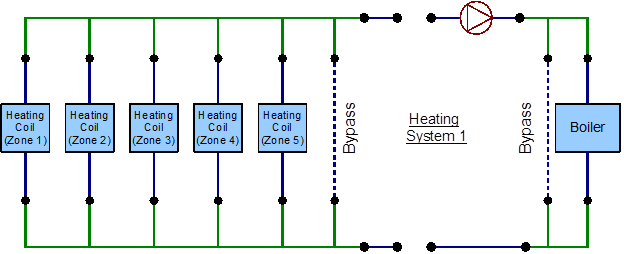
\includegraphics[width=0.9\textwidth, height=0.9\textheight, keepaspectratio=true]{media/image044.png}
\caption{EnergyPlus line diagram for heating loop \protect \label{fig:energyplus-line-diagram-for-heating-loop}}
\end{figure}

SHWSys1

The cooling side of the system will be modeled first. The primary cooling loop (named ``CoolSysPrimary'' in the input file) uses the chiller as the supply side component to charge the TES tank. The chilled water that is stored in the TES tank is then supplied to the cooling coil. A cooling tower that operates on the supply side of the condenser loop (named ``Condenser Loop'') supplies the cooling water to the chiller that is used in the primary cooling loop. These two loops serve as the cooling system for this building. This system will be modeled first with emphasis placed on the primary cooling loop. In particular the schedules used for the charging and discharging the TES tank play a crucial role in the efficient operation of the system.

The building also has one heating loop. The heating loop (named ``HeatSys 1'') uses a boiler to provide hot water to five heating coils that are located in the five zones. This heating loop also supplies hot water to the reheat coil. A flow chart for loop identification is provided in Figure~\ref{fig:flowchart-for-loop-identification-001}.

\begin{figure}[hbtp] % fig 45
\centering
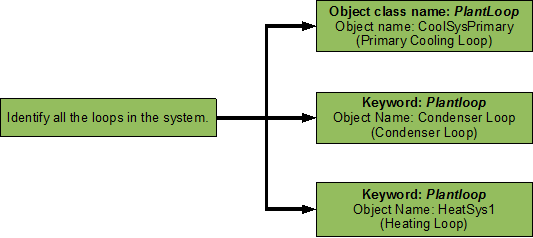
\includegraphics[width=0.9\textwidth, height=0.9\textheight, keepaspectratio=true]{media/image045.png}
\caption{Flowchart for loop identification \protect \label{fig:flowchart-for-loop-identification-001}}
\end{figure}
